\chapter{Space segment}
The space segment is a part of the satellite communication system that resides on the satellite itself. It is divided into two main parts: a communication subsystem (COMM) and antennas (ANTs) connected with two coaxial cables. The space segment is critical in system operation and reliability - there is no possibility to carry out any repairs, perform maintenance or adjustment once on orbit. It is exposed to space environment – with wide temperature range, thermal cycling, cosmic radiation and vacuum. To improve reliability, it was decided to choose commercially available and flight-proven CubeSat components to increase the overall reliability of the system.

\section{Flatsat}
Most of the tests were performed on Flatsat (an abbreviation from Flat Satellite), an electronic test bench, which consists of a mix of flight models, engineering models of the instruments and Electrical Ground Support Equipment (EGSE). EGSE are the test instruments and mocks (fake) instruments, which allow testing without the need for actual hardware. PW-Sat2 Flatsat was integrated in the Space Research Centre in Warsaw. Flatsat is shown in figure \ref{flatsat_photo}. To perform the communication tests, a Ground Station mock was created on the flatsat. It was built using to Software-Defined Radios: one, as downlink receiver, same as to be installed in the Ground Station, and the second to generate uplink signals. Use of SDR instead of analogue radio transceiver greatly simplified the tests performed.

\begin{figure}[H]
    \centering
    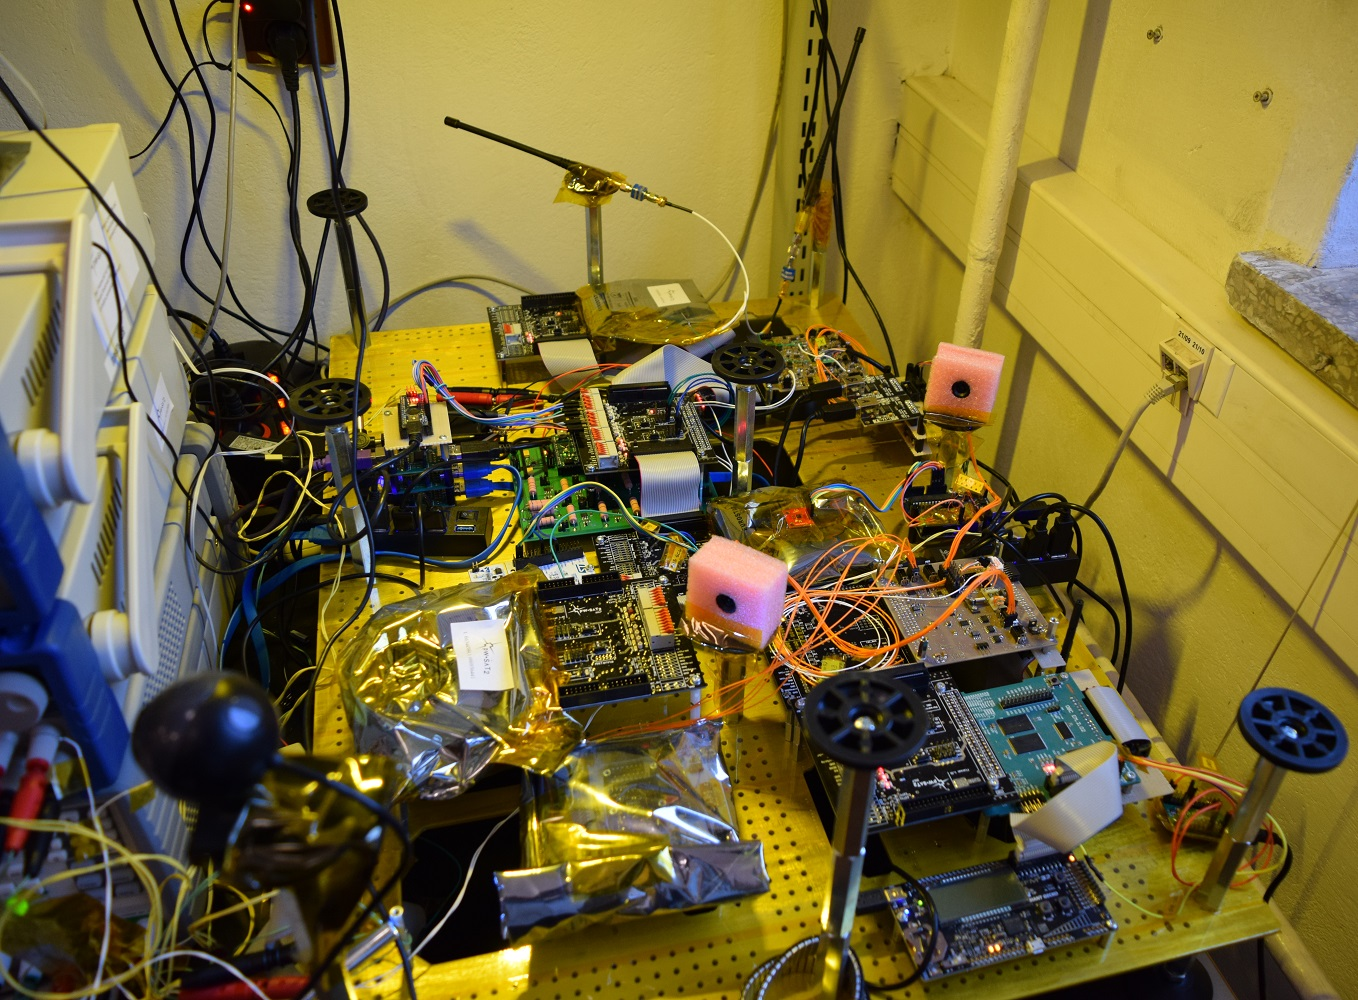
\includegraphics[width=0.48\paperwidth]{img/6/flatsat.jpg}
    \caption{PW-Sat2 flatsat in Space Research Centre, Warsaw}
    \label{flatsat_photo}
\end{figure}

% -----------------------------------------------------------------------------------------------------------
% -----------------------------------------------------------------------------------------------------------
% -----------------------------------------------------------------------------------------------------------

\section{Spacecraft communication transceiver}
\label{section:comm_design}
CubeSat design specification \cite{cubesat_spec}, with which PW-Sat2 is compliant, defines common PC/104 connector, which is the main data bus for all satellite subsystems. On the connector, two \iic and two CAN buses are defined, and most of the components are compatible with each other. However, due to the lack of CAN interface on the On-Board Computer (CubeComputer from CubeSpace \cite{cubespace_website}) radio should use \iic communication bus.

When the subsystem was ordered (in year \si{2014}), the choice of available products was very limited, and the only radio which was compliant with above-mentioned requirements was ISIS VHF uplink/UHF downlink Full Duplex Transceiver. Its view and block diagram is shown in the figures \ref{ISIS_TRXvU_photo} and \ref{ISIS_TRXvU_block_diagram}. Basic characteristics of the communications module are shown in table \ref{isis_comm_params}.

\begin{figure}[H]
    \centering
    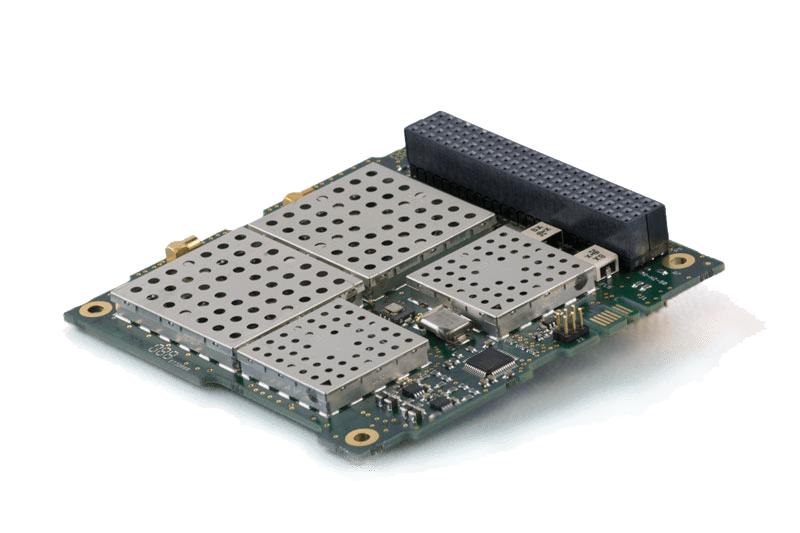
\includegraphics[width=0.7\paperwidth]{img/6/ISIS-radio-UHF-VHF-min.png}
    \caption{ISIS VHF uplink/UHF downlink Full Duplex Transceiver photo. Source: \cite{isis_trxvu}}
    \label{ISIS_TRXvU_photo}
\end{figure}

\begin{figure}
    \centering
    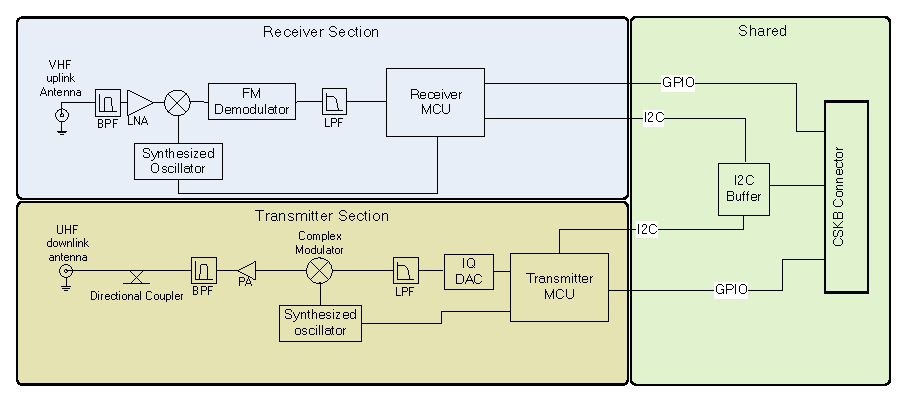
\includegraphics[width=0.8\paperwidth]{img/6/ISIS_TRXvU_block_diagram.eps}
    \caption{ISIS VHF uplink/UHF downlink Full Duplex Transceiver block diagram. Source: \cite{isis_trxvu}}
    \label{ISIS_TRXvU_block_diagram}
\end{figure}

\begin{table}[H]
\small
\centering
\caption{ISIS VHF uplink/UHF downlink Full Duplex Transceiver parameters}
\label{isis_comm_params}
\arrayrulecolor{black}
\begin{tabular}{c|c}
     \textbf{downlink} & \textbf{uplink} \\ \hline
     \multicolumn{2}{c}{dual-\iic ~communication standard} \\
     \multicolumn{2}{c}{AX.25 frame format} \\
     \si{430}-\SI{450}{\MHz} frequency range & \si{140}-\SI{150}{\MHz} frequency range \\
     \SI{0.5}{\watt} downlink power & \SI{-98}{\dBm} sensitivity for \si{10^-5}~BER \\
     \si{1.2} - \SI{9.6}{\kilo\bit / \second} bitrate & \SI{1.2}{\kilo\bit / \second} bitrate \\ 
     BPSK modulation with G3RUH scrambling & FM-modulated AFSK \\ 
\end{tabular}
\end{table}

\vspace{0.5cm}

The transceiver was tested separately for its uplink and downlink capabilities. Tests are critical to make sure that radio parameters are maintained in the system and to verify the manufacturers' data.

\subsection{Sensitivity measurement}
Sensitivity is the minimal input power to the receiver on which it receives the packets correctly. This parameter depends on the receiver construction, Noise Factor of the amplifiers and the demodulator itself. Sensitivity was measured by the setup shown in the figure \ref{4_uplink_sensitivity}. During the test measurement, the input noise on the receiver port is only Johnson-Nyquist noise and transmitter impairments, without accounting for the antenna-added terrestrial noise. For the final application, the antenna temperature has to be taken into account, increasing the spectral noise density on the receiver port.

Sensitivity test procedure:
\begin{itemize}
    \item measuring output power of PlutoSDR using spectrum analyzer with wide RBW filter (\SI{1}{\MHz}),
    \item calculating input power to the Communications module,
    \item PER is calculated by transmitting \si{1000} data frames using PlutoSDR (with GNUradio) and receiving them by the On-Board Computer connected to the PC, the output power of PlutoSDR was regulated for each data point.
\end{itemize}

\begin{figure}[h]
    \centering
    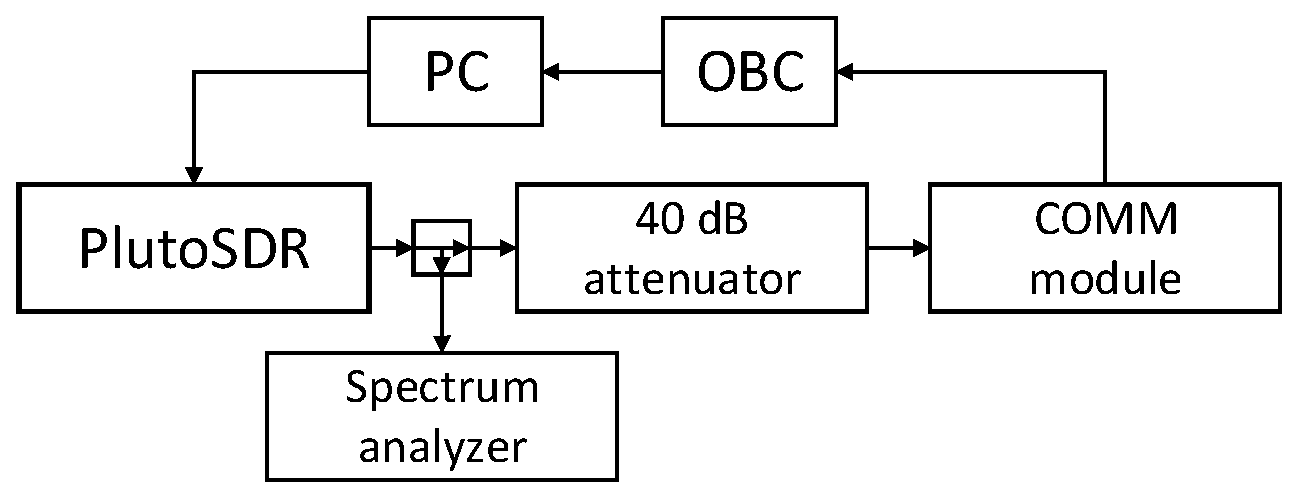
\includegraphics[width=0.6\paperwidth]{img/6/uplink_sensitivity.eps}
    \caption{Uplink sensitivity measurement block diagram}
    \label{4_uplink_sensitivity}
\end{figure}

Measured PER chart is shown in the figure \ref{4_uplink_sensitivity_graph}. It is compared to the ideal BFSK curve. For assumed usable PER of about \SI{1}{\percent}, the sensitivity of the communication module is \SI{-97}{\dBm}.

\begin{figure}[H]
    \centering
    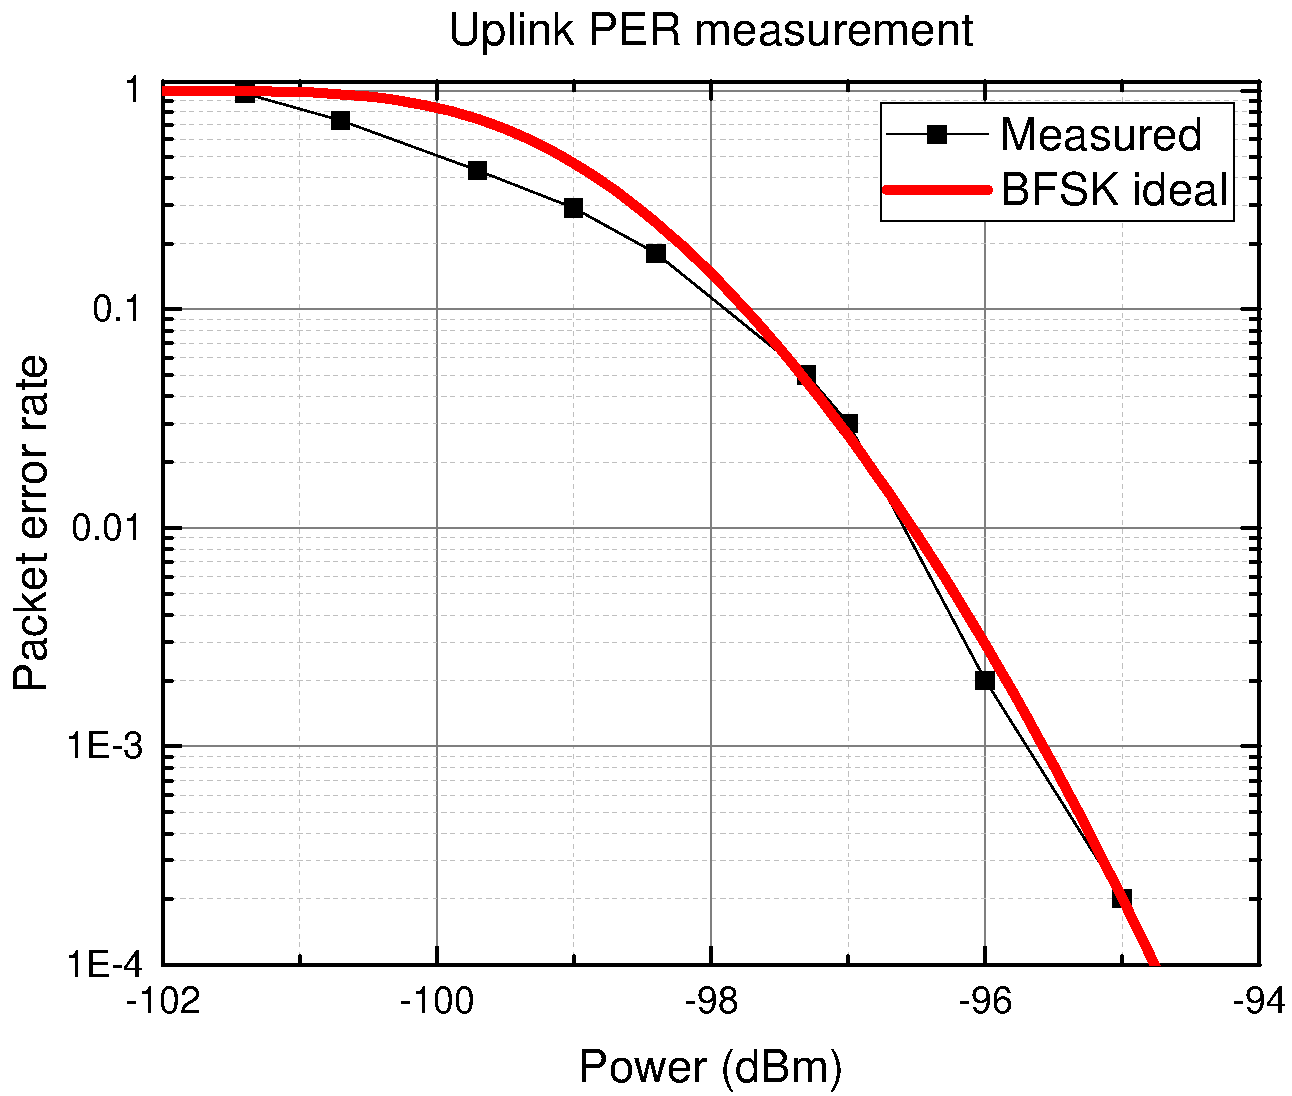
\includegraphics[width=0.8\paperwidth]{img/6/uplink_per.pdf}
    \caption{Uplink sensitivity measurement}
    \label{4_uplink_sensitivity_graph}
\end{figure}


\subsection{Doppler effect influence on uplink}
Doppler effect is caused when a fast-moving object is emitting/receiving waves, such as acoustic or radio frequencies. For uplink frequency (VHF band) Doppler effect can shift received frequency up to about \SI{5}{\kHz}. The receiver bandwidth should be measured to estimate allowable frequency inaccuracies.

The test setup is the same as in the previous setup, shown in the figure \ref{4_uplink_sensitivity}. During the test, the PER was measured for a range of frequency offsets from the center frequency of the module. The input power to the module was set to \SI{3}{\dB} above sensitivity level (\SI{-94}{\dBm}). The result is shown in figure \ref{4_uplink_doppler_measurement}.
\begin{figure}[H]
    \centering
    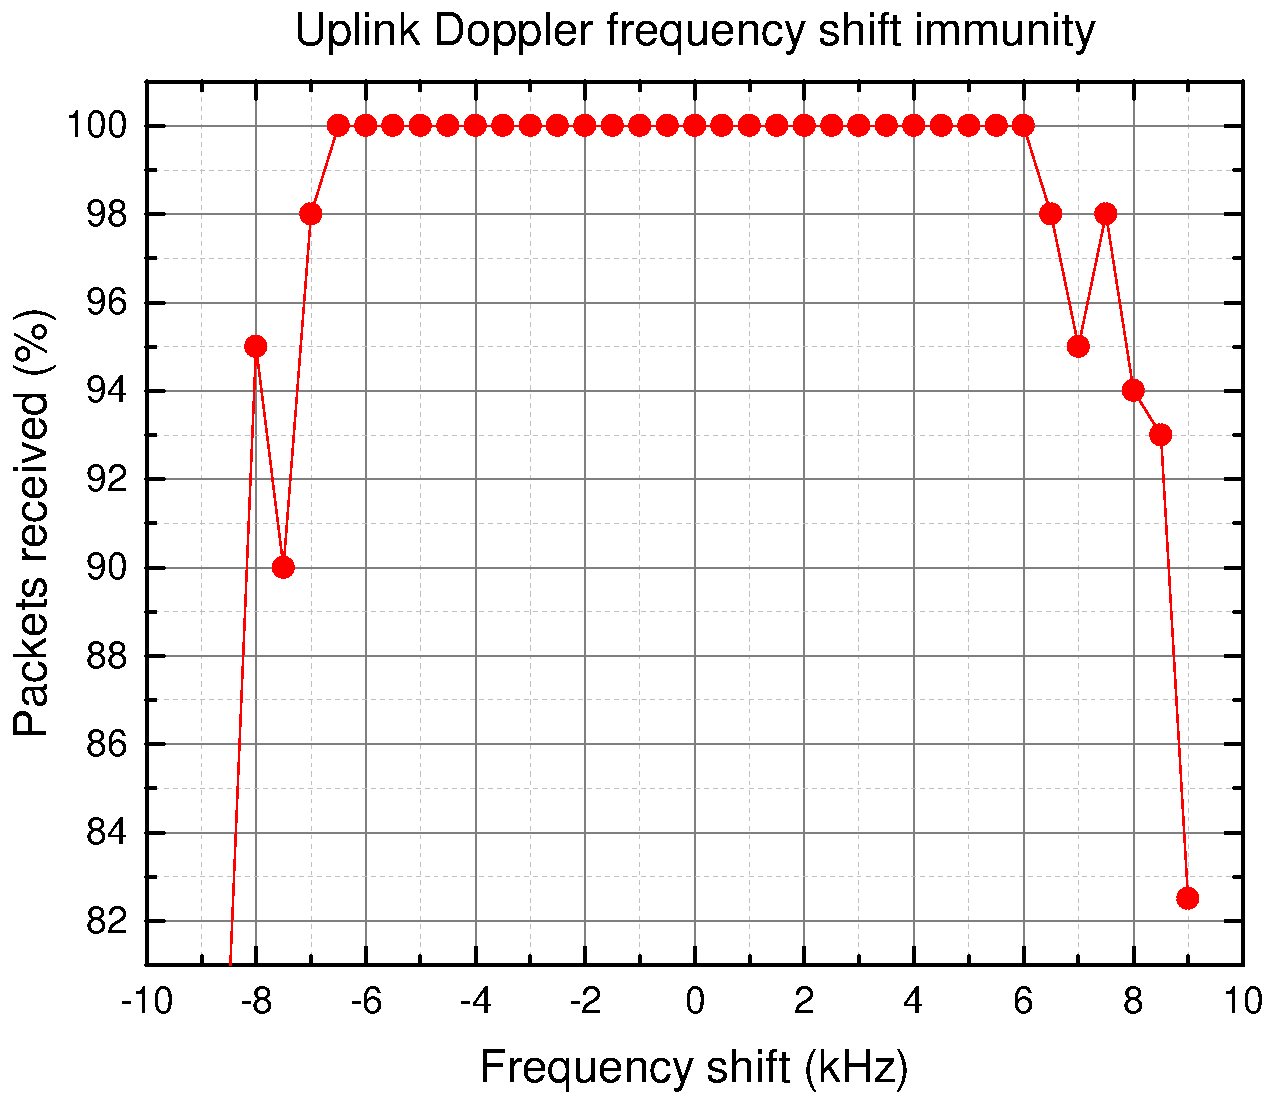
\includegraphics[width=0.6\paperwidth]{img/6/uplink_doppler.pdf}
    \caption{Uplink Doppler effect influence measurement}
    \label{4_uplink_doppler_measurement}
\end{figure}


\subsection{Transmitter spectrum and output power}
Output power was measured using spectrum analyzer with wide resolution bandwidth. Output power was measured to be \SI{28}{\dBm}, which is within the manufacturer specification.
The spectrum of the signal was recorded (fig. \ref{tx_spectrum}), showing significant side lobes (first lobe \SI{18}{\dB} lower than main carrier).

\begin{figure}[H]
    \centering
    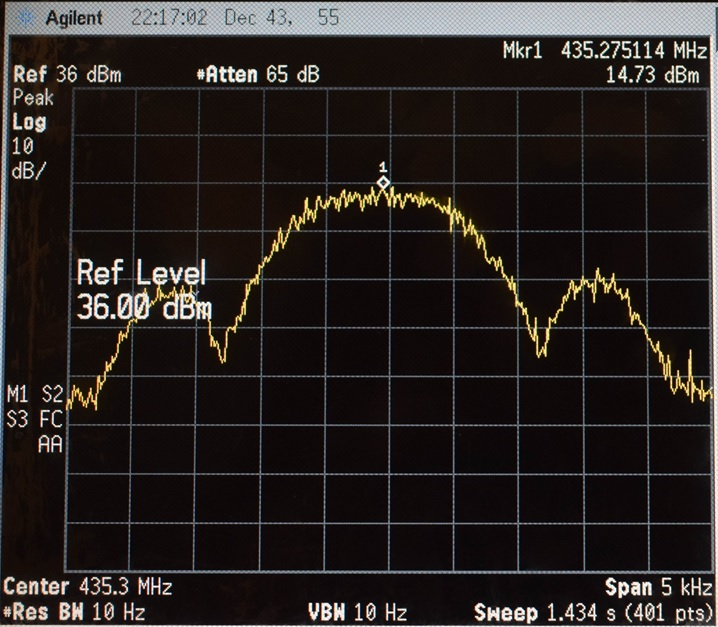
\includegraphics[width=0.6\paperwidth]{img/6/tx_spectrum.jpg}
    \caption{Communications module transmit spectrum}
    \label{tx_spectrum}
\end{figure}






% -----------------------------------------------------------------------------------------------------------
% -----------------------------------------------------------------------------------------------------------
% -----------------------------------------------------------------------------------------------------------



\section{Spacecraft Antennas}
Because of the selected radio system, two antennas have to be installed - one for uplink (VHF) and one for downlink (UHF). Antennas should be omnidirectional, as PW-Sat2 does not have a nadir-pointing capability and random tumbling during operation is assumed.

Self-made dipole antenna was considered at the design stage, but due to mechanical and time constraints, satellite antenna was decided to be bought as well. Innovative Solutions In Space company sells antenna with the transceiver as CubeSat communication Kit \texttt{CubeSat dipole antenna system}. Both elements are compatible and the whole system (transceiver + antenna) is tuned for specific communication frequency and mounting option.

This system is deployable by the command from the On-Board Computer. Thermal knife (resistor) is heated up, and the thermal link is burnt, resulting is antenna deploy by the spring action. Figure \ref{ISIS_antenna} shows an antenna system.

\begin{figure*}
   \centering
\begin{tabular}{cc}
        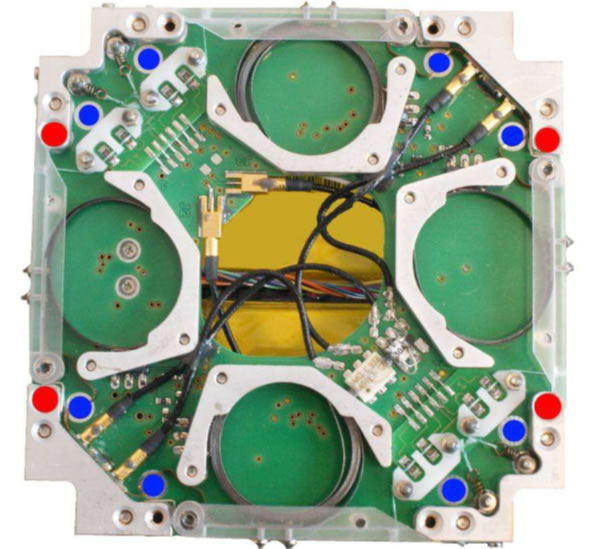
\includegraphics[width=0.3\paperwidth]{img/6/isis_antenna_stowed.jpg}
    & 
        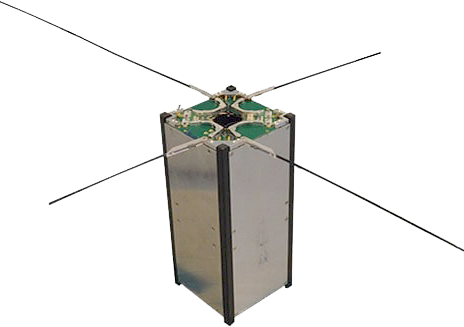
\includegraphics[width=0.45\paperwidth]{img/6/CubeSat-antenna-dipole-configuration.png}    
\end{tabular}
\label{ISIS_antenna}
\caption{ISIS CubeSat dipole antenna system in stowed and deployed position. Source: \cite{isis_dipole_antenna}}
\end{figure*}


\subsection{Tests}
The first automatic task of the satellite it to deploy the antennas. During the test campaign, antenna deployment procedure was executed four times, due to the issues with Antenna opening. In figure \ref{pwsat_with_deployed_antennas} the satellite during antenna deployment is shown.

\begin{figure}
    \centering
    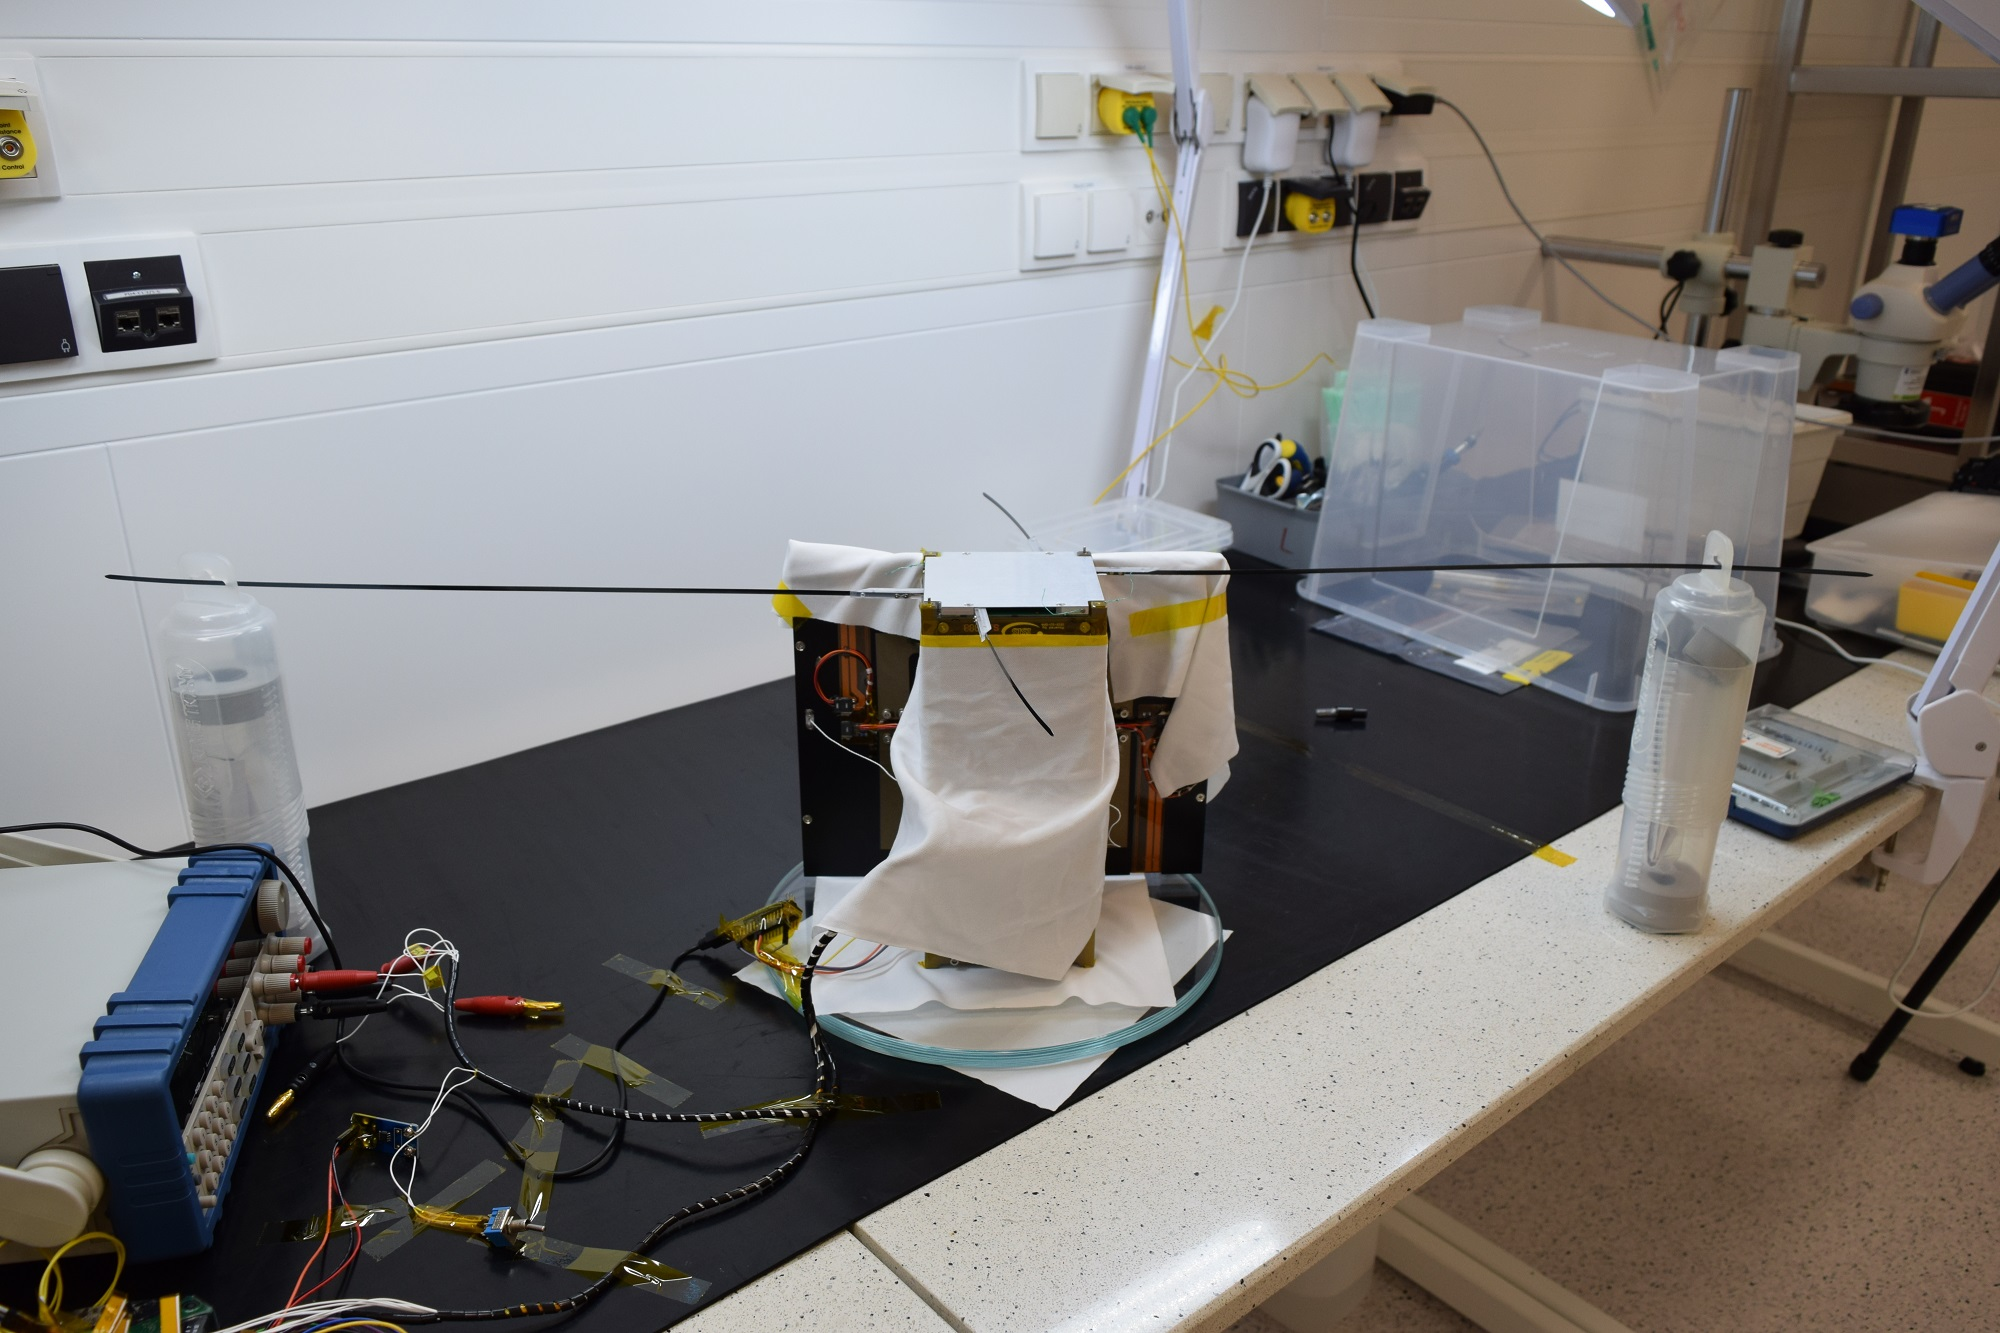
\includegraphics[width=0.8\paperwidth]{img/6/pwsat_with_deployed_antennas.JPG}
    \caption{PW-Sat2 with deployed solar panels during antenna verification}
    \label{pwsat_with_deployed_antennas}
\end{figure}

Manufacturer of the antennas provides a test report with the measured antennas matching ($s_{11}$ parameter), for VHF and UHF frequencies they are shown in figures \ref{isis_s11_vhf} and \ref{isis_s11_uhf}, respectively.

\begin{figure}[H]
    \centering
    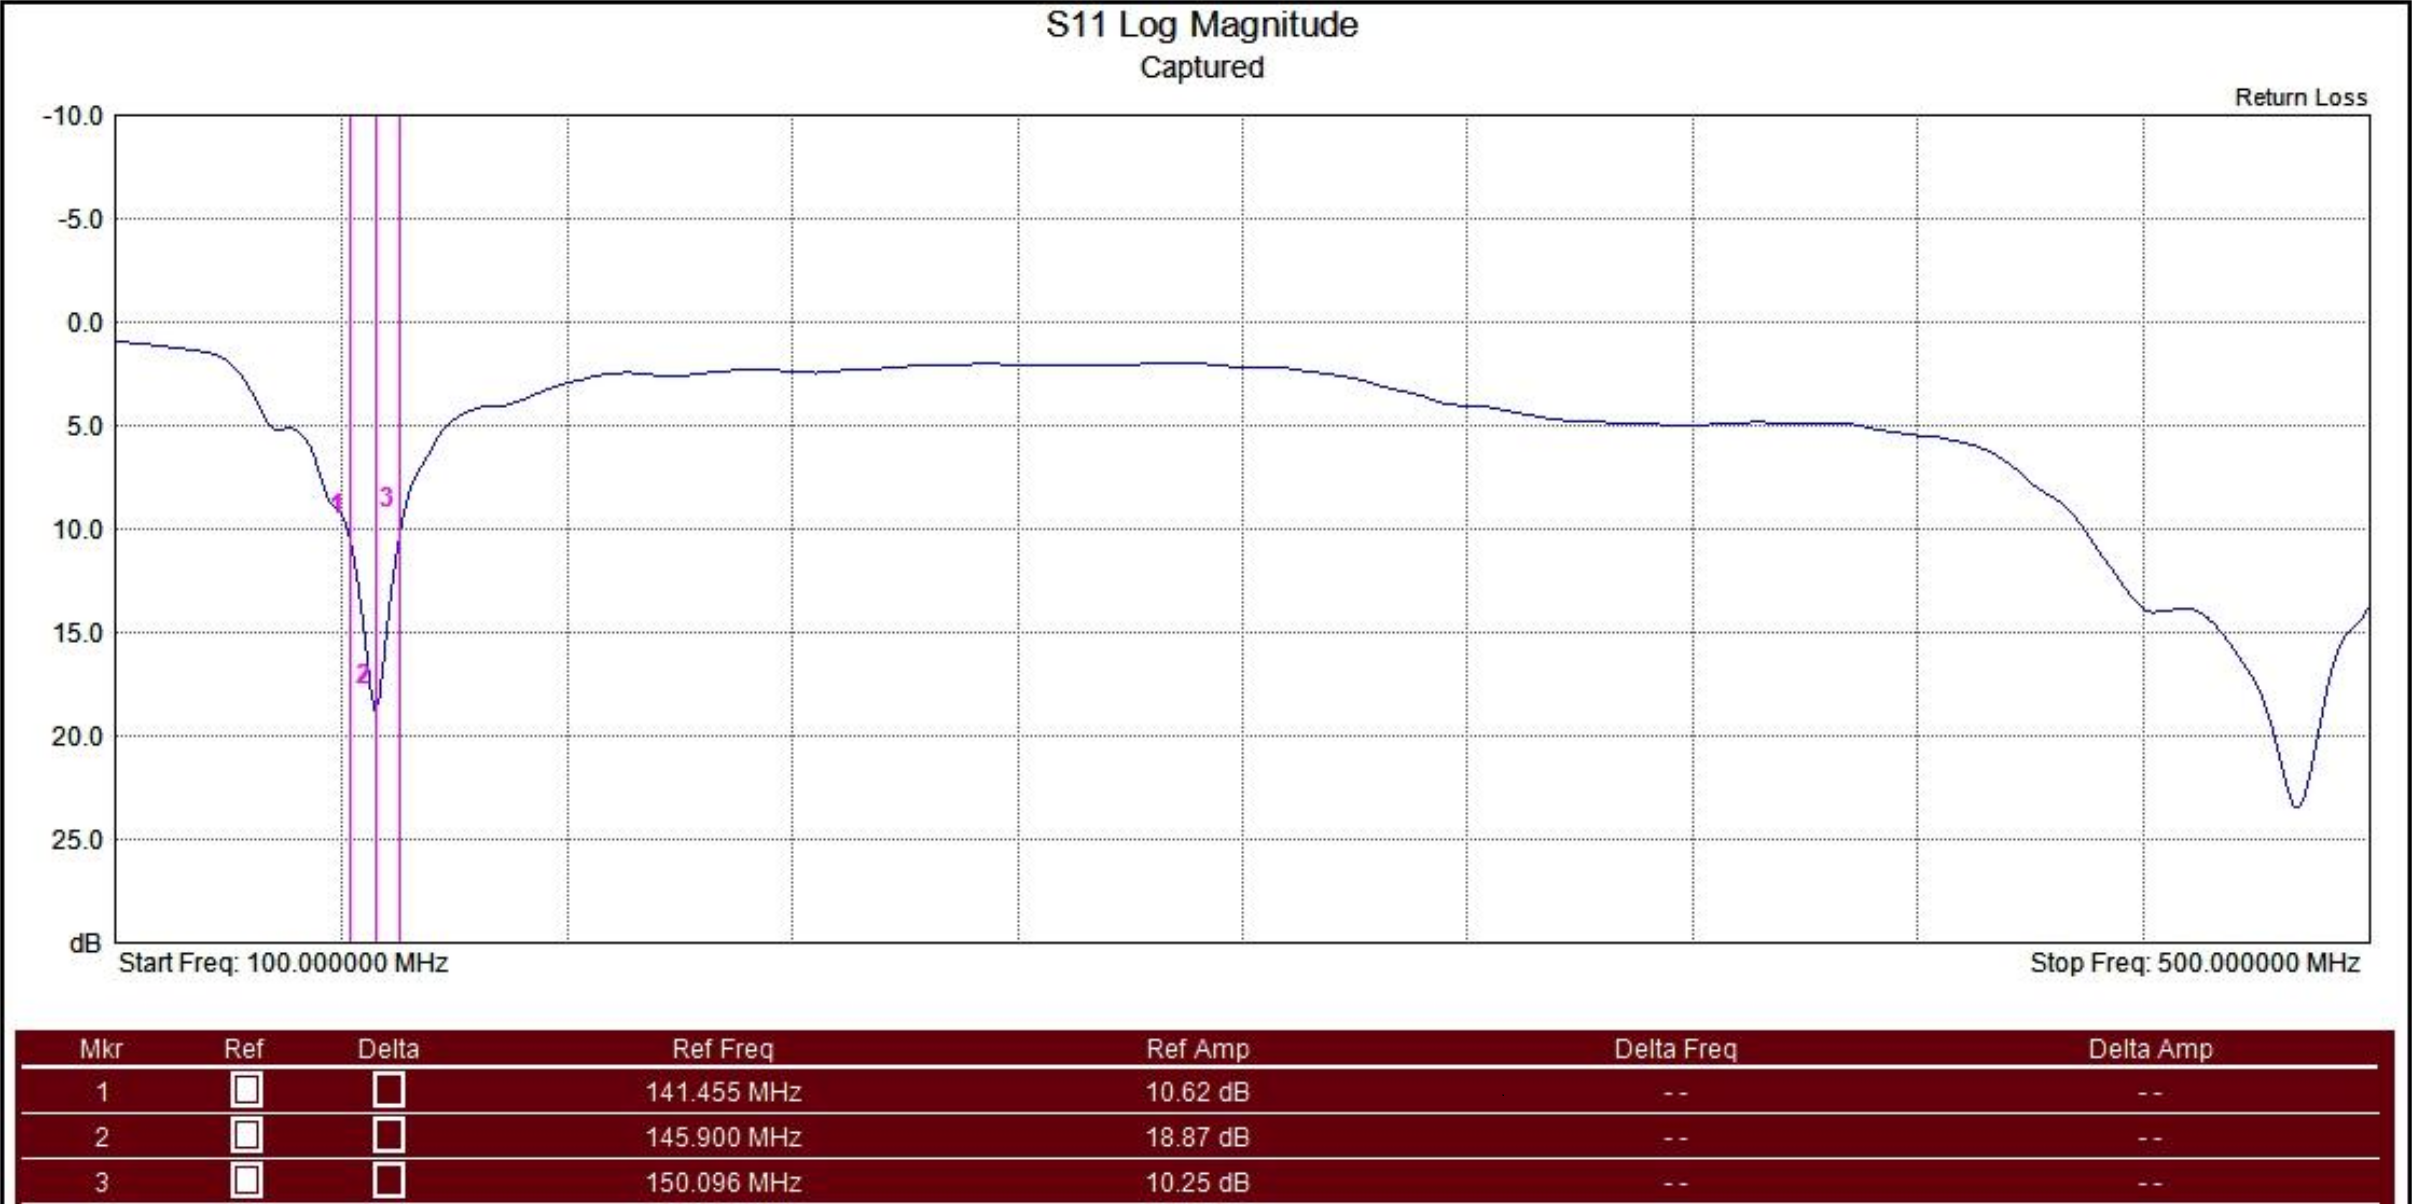
\includegraphics[width=0.8\paperwidth]{img/6/isis_s11_vhf.png}
    \caption{VHF antenna matching. Source: \cite{isis_ant_test_report}}
    \label{isis_s11_vhf}
\end{figure}

\begin{figure}[H]
    \centering
    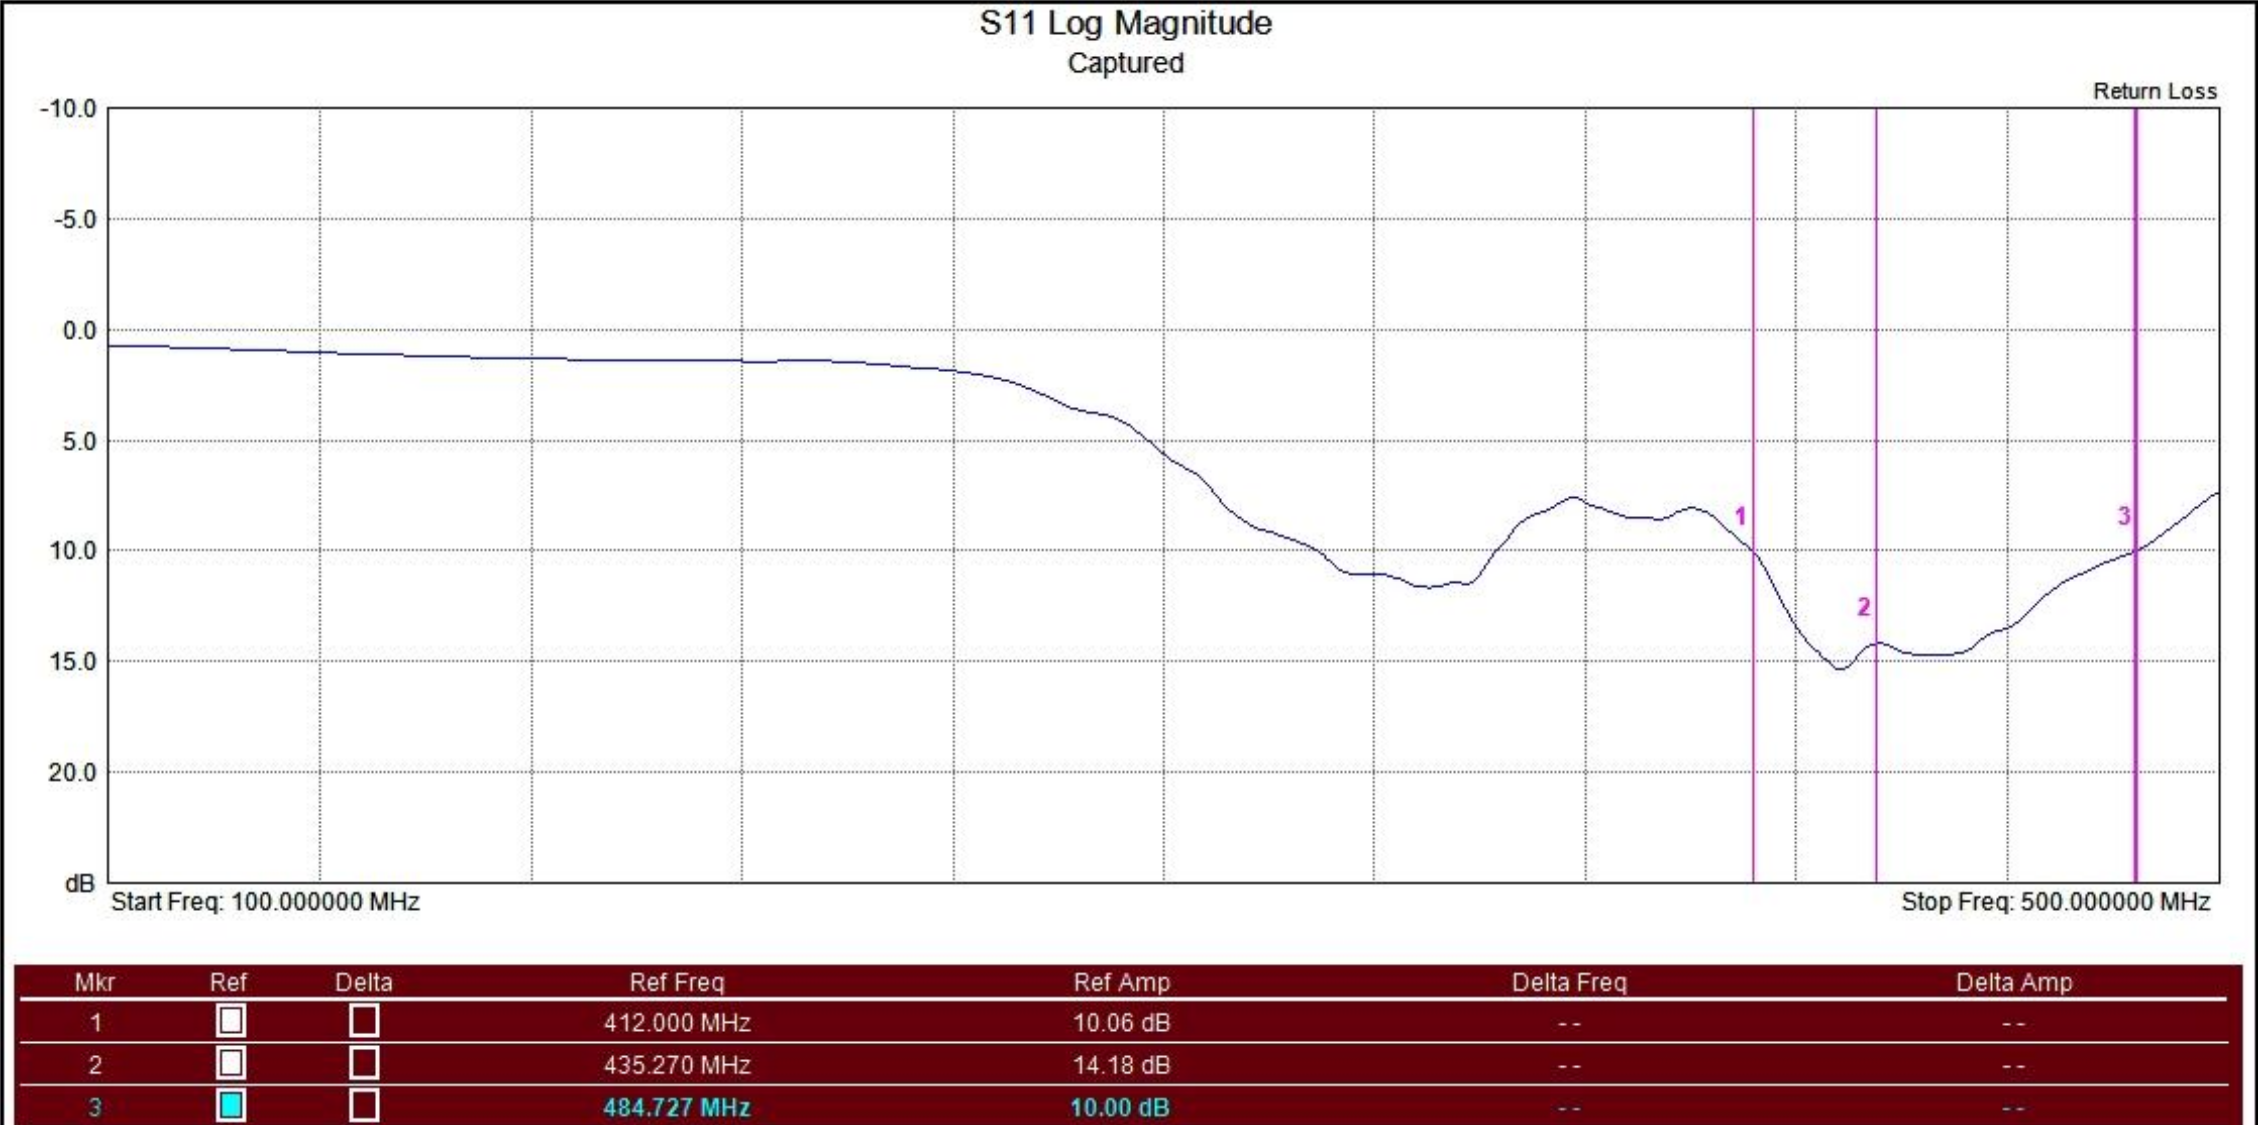
\includegraphics[width=0.8\paperwidth]{img/6/isis_s11_uhf.png}
    \caption{UHF antenna matching. Source: \cite{isis_ant_test_report}}
    \label{isis_s11_uhf}
\end{figure}

\newpage

Both forward and reflected power from the antenna are measured by the radio module during radio frame transmission. Correct antenna deployment can be verified also by using the telemetry. During the test antenna deployment both forward and reflected power were captured. Average measured value of the forward power: \textbf{\SI{28.8}{\dBm} $\pm$ \SI{0.43}{\dBm}} and reflected power: \textbf{\SI{19.6}{\dBm} $\pm$ \SI{0.54}{\dBm}}. This means that the antenna matching for UHF frequencies is: SWR~$= 2.1$, $s_{11} = -9.2~dB$. This means that the power lost in the mismatch is \SI{0.5}{\dB}. Measured value is similar to measured by the manufacturer ($s_{11} = \SI{-14}{\dB}$).

\subsection{Antennas on orbit}
Reflected and forward powers are being measured throughout the mission, the chart of the reflected and forward power, from the ground testing up to mission completion is shown in the figure \ref{4_rf_power_comm}. This graph shows that VSWR of the antenna did not change much during the mission. However, Sail and Solar Arrays deployments can be clearly seen on the measurements. Picture of the shadow of the satellite on the Sail, showing opened antennas is shown in figure \ref{antennas_deployed_orbit}.

\begin{figure}[H]
    \centering
    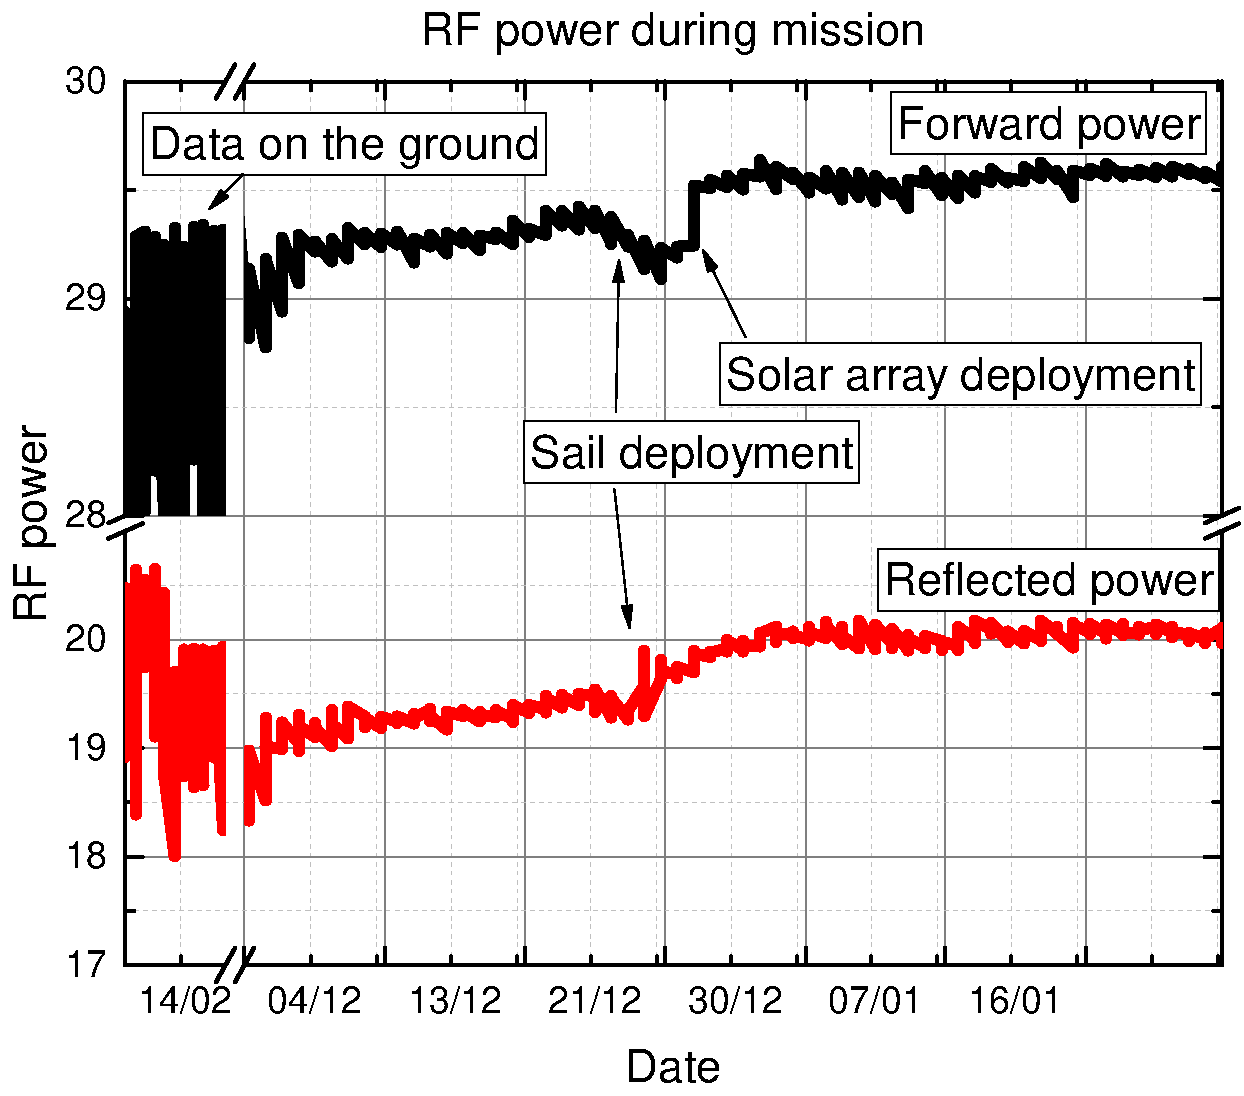
\includegraphics[width=0.6\paperwidth]{img/6/rf_power_comm.pdf}
    \caption{RF power during mission}
    \label{4_rf_power_comm}
\end{figure}

\begin{figure}
    \centering
    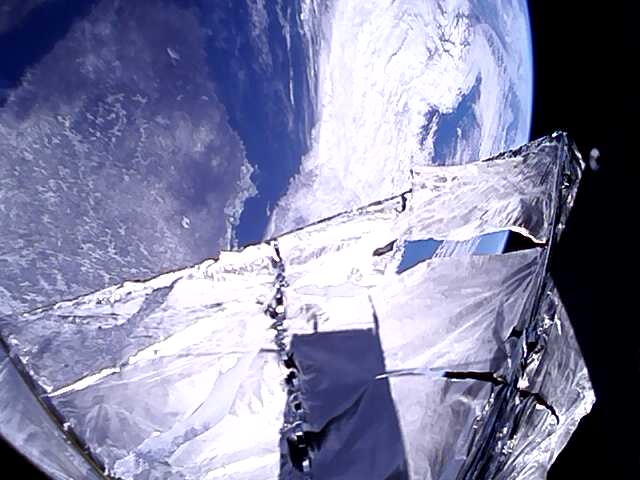
\includegraphics[width=0.7\paperwidth]{img/6/antennas_deployed_orbit.jpg}
    \caption{On-Board photo from PW-Sat2 showing opened antennas}
    \label{antennas_deployed_orbit}
\end{figure}


% -----------------------------------------------------------------------------------------------------------
% -----------------------------------------------------------------------------------------------------------
% -----------------------------------------------------------------------------------------------------------

% \subsubsection{Deployable elements influence on the antenna pattern}
% TODO

% On-board PW-Sat2 are two main deployables: solar panels and deorbitation sail.

% During the design stage, the influence of the solar panels was discussed with antenna manufacturer - the outcome was to place longed dipoles (VHF) along with the solar panels, and shorter ones orthogonally to it, as shown in the figure \ref{???}

% % TODO: zdjęcie z otwartymi panelami i antenami

% The influence of the deorbit sail was also simulated during Critical Design stage.

% Deorbitation sail is made by very thin (\SI{5}{\micro\meter}) mylar foil with aluminum coating. Using % TODO
% simulation tool, it was shown that the sail would increase the directivity of the CubeSat antennas, acting as a reflector.
% % TODO: jakieś zdjęcie z symulacji, wynik o ile dB się pogorszyło


